\documentclass{article}

\usepackage{amsmath,amssymb,amsfonts}
\usepackage{graphicx}
\usepackage{float}
\usepackage{geometry}
\usepackage{subcaption}

\usepackage{wrapfig}

\begin{document}

\title{Zlepki nad triangulacijami - DN 8}
\maketitle

Uporabljeni MATLAB fajli iz prejšnjih nalog:
\begin{itemize}
\item bpolyval.m - izračuna vrednost polinoma v Bernstein-Bezier repr.
\item changeBasis.m - Izračuna koeficiente polinoma v drugem baricentričnem ogrodju.
\item checkSmoothnessSpline.m - Izračuna red gladkosti med trikotniki.
\item coeffSmoothness.m - Določi koeficiente potrebne za dan red gladkosti.
\item constructSpline.m - iz podatkov ($\alpha$) izračuna zlepek (koeficiente nad vsakim trikotnikom)
\item constructSplineFromFunc.m - izračuna zlepek iz funkcije
\item decasteljau.m - decasteljau-ev algoritem (splošen)
\item evaluateSpline.m - izračuna vrednost zlepka nad triangulacijo v dani točki.
\item getLinfError - Izračuna l-inf napako za dano aproksimacijo.
\item interpolation.m - interpolira podatke (vrednosti + grad) na trikotniku.
\end{itemize}

Novi fajli:
\begin{itemize}
\item boundaryEdge.m - Preveri če je dana stranica na robu domene.
\item constructSplineCloughTocher.m
\item constructSplineFoleyOpitz.m
\item constructSplineFromFuncCloughTocher.m
\item constructSplineFromFuncFoleyOpitz.m
\item gammaFunctional.m - Izračuna tisti gamma člen
\item getOpposite.m - za dano triangulacijo vrne "nasprotni" vertex (če imamo trikotnika ki se stikata)
\item thirdTerm.m - Izračuna 3. člen v (1,1,1) formuli v Clough Tocher
\item testHW8.m - skripta, ki prikaže rezultate prikazane v tem pdf-u
\end{itemize}



Primerjali bomo 3 metode aproksimacije:
\begin{itemize}
\item Naivna metoda iz naloge 6, kjer preostali koeficient določimo malo bolj arbitrarno. To smo že vidili je $C^0$ zlepek.
\item Foley-Opitz makro-element. V teoriji je tudi to $C^0$ zlepek, kar tudi moja koda potrdi. Red konvergence je večji v primerjavi s prejšnjo metodo - naklon je večji od $3$. V contourju lahko levo spodaj npr. vidimo, da se zlepek nekoliko lepše obnaša.
\item Clough-Tocher makro-element. V teoriji je $C^1$ zlepek, moja koda (matrike sem primerjal do tolerance 1e-10) to tudi potrdi za večino stranic, vendar so nekatere tudi gladke ali celo nezvezne. Verjetno je v določitvi enega izmed koeficientov kakšen typo, a ga nisem našel. Naklon pri napaki je spet večji od $3$. Večja gladkost zlepka se vidi na contourjih na sredini-levo od sredine. Ti rezultati niso končni za to metodo, saj vem, da je nekje šlo nekaj narobe (glede na to, da imamo prisotne stranice, kjer je zlepek nezvezen).
\end{itemize}
\begin{figure}[H]
\centering
\begin{subfigure}{.3\textwidth}
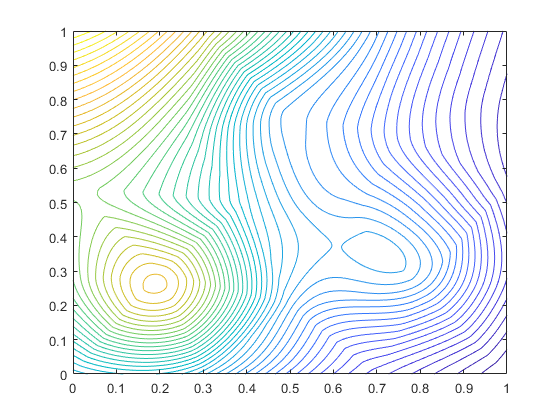
\includegraphics[width=\linewidth]{slike/contour1.png}
\end{subfigure}
\begin{subfigure}{.3\textwidth}
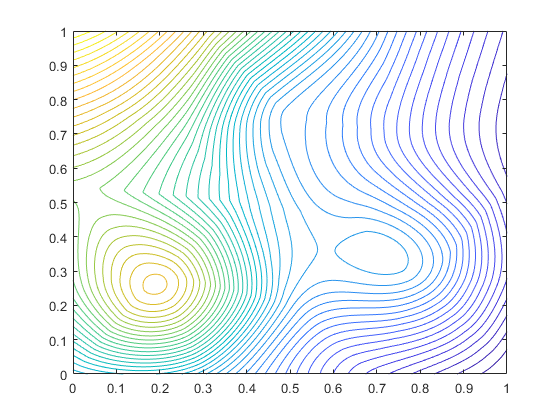
\includegraphics[width=\linewidth]{slike/contour2.png}
\end{subfigure}
\begin{subfigure}{.3\textwidth}
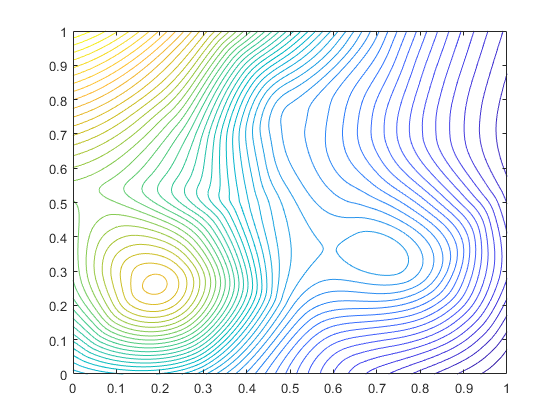
\includegraphics[width=\linewidth]{slike/contour3.png}
\end{subfigure}
\caption*{Contouri za naivno, Foley-Opitz, Clough-Tocher.}
\end{figure}

\begin{figure}[H]
\centering
\begin{subfigure}{.3\textwidth}
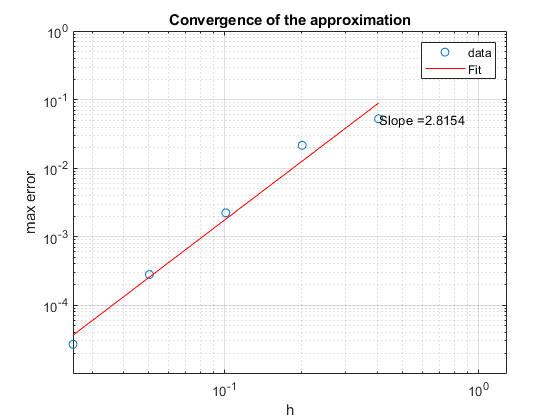
\includegraphics[width=\linewidth]{slike/conv1.png}
\end{subfigure}
\begin{subfigure}{.3\textwidth}
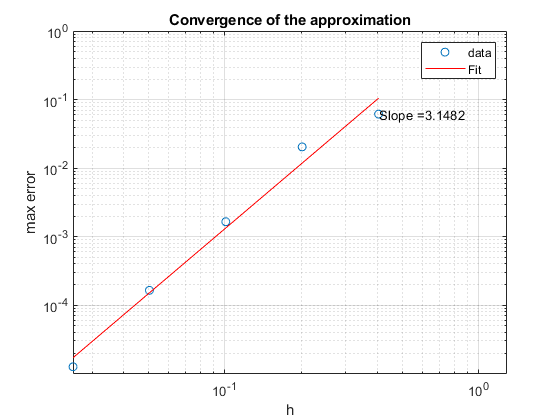
\includegraphics[width=\linewidth]{slike/conv2.png}
\end{subfigure}
\begin{subfigure}{.3\textwidth}
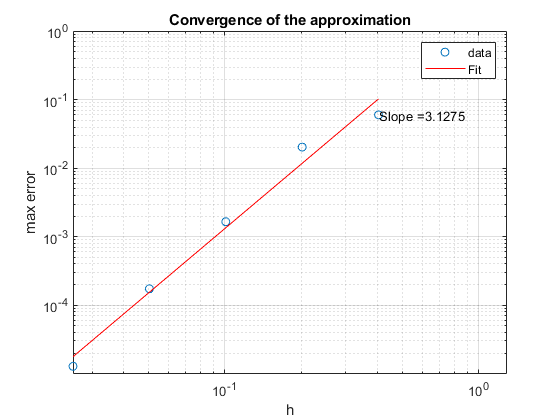
\includegraphics[width=\linewidth]{slike/conv3.png}
\end{subfigure}
\caption*{Konvergenca za naivno, Foley-Opitz, Clough-Tocher.}
\end{figure}
\end{document}
